\chapter{Γεννήτρια Χωροχρονικών Δεδομένων}

\section{Αποθήκευση Χωρικών Δεδομένων}

Η γεννήτρια χωροχρονικών δεδομένων χρησιμοποιεί πραγματικά σημεία ενδιαφέροντος στο χάρτη ως πηγή χωρικών δεδομένων, όπως αυτά εμφανίζονται σε διαδικτυακές υπηρεσίες 
συστημάτων προτάσεων (recommendation systems) σαν το TripAdvisor \cite{1}. Τα σημεία αυτά αναγνωρίζονται από τις γεωγραφικές συντεταγμένες τους καθώς και τη 
διεύθυνση τους στο χάρτη. Επίσης, συνοδεύονται από βαθμολογίες και κριτικές, οι οποίες έχουν γίνει από χρήστες της υπηρεσίας TripAdvisor. Το πλήθος των  
διαθέσιμων σημείων ενδιαφέροντος για τη δημιουργία της γεννήτριας χωροχρονικών δεδομένων ανέρχεται σε σύνολο 136409 σημείων, τα οποία προέκυψαν από αρχείο 
μεγέθους 13GB. Για την αποθήκευσή τους χρησιμοποιήθηκε 
η σχεσιακή βάση δεδομένων PostgreSQL. Το σχήμα της βάσης περιλαμβάνει δύο πίνακες, έναν για τα σημεία ενδαφέροντος και τα χαρακτηριστικά τους και έναν για τις κριτικές και 
βαθμολογίες που έχουν γίνει στα σημεία αυτά. 

\begin{figure}[H]
  \centering
  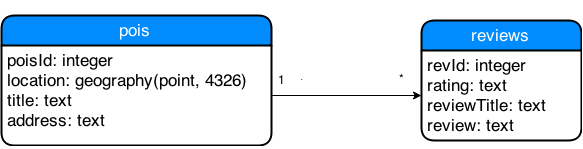
\includegraphics[width=0.7\textwidth]{figures/schema.png}
  \caption{Σχήμα βάσης δεδομένων για τα χωρικά δεδομένα}
\end{figure}

Πιο αναλυτικά, ο πίνακας για τα σημεία ενδιαφέροντος περιέχει τα εξής γνωρίσματα:

\begin{itemize}
 \item poisId: αναγνωριστικός ακέραιος αριθμός του σημείου ενδιαφέροντος, κύριο κλειδί.
 \item location: οι γεωγραφικές συντεταγμένες του σημείου. Χρήση του γεωγραφικού τύπου δεδομένων ο οποίος υποστηρίζεται από την επέκταση PostGIS της PostgreSQL.
 \item title: η ονομασία του σημείου.
 \item address: η διεύθυνση του σημείου.
\end{itemize}

Ένα σημείο ενδιαφέροντος μπορεί να έχει πολλές κριτικές, γι'αυτό και οι δύο πίνακες συνδέονται με σχέση 1 προς πολλά. Ο πίνακας για τις κριτικές περιέχει τα εξής 
γνωρίσματα:

\begin{itemize}
 \item revId: αναγνωριστικός ακέραιος αριθμός του σημείου ενδιαφέροντος στο οποίο αντιστοιχεί η κριτική, εξωτερικό κλειδί.
 \item rating: βαθμολογία του σημείου σε κλίμακα ακεραίων 1 έως 5.
 \item reviewTitle: ο τίτλος της κριτικής για το σημείο.
 \item review: το κείμενο της κριτικής για το σημείο.
\end{itemize}

Μετά την αποθήκευση όλων των διαθέσιμων χωρικών δεδομένων αναθέτουμε ένα ευρετήριο τύπου B-tree στο γνώρισμα poisId του πίνακα pois και στο γνώρισμα revId του πίνακα 
reviews. Επίσης, δημιουργούμε ένα ευρετήριο τύπου GiST στο γνώρισμα location του πίνακα pois. Με τις δομές αυτές θα μπορεί να γίνει αποδοτικά η αναζήτηση 
εγγραφών ως προς τους αναγνωριστικούς τους αριθμούς αλλά και ως προς την τοποθεσία ενός σημείου ενδιαφέροντος. 

\section{Παράμετροι Εισόδου Γεννήτριας}

Η γεννήτρια χωροχρονικών δεδομένων λαμβάνεις τις εξής παραμέτρους εισόδου:

\begin{itemize}
 \item userIdStart: Ο αναγνωριστικός αριθμός του πρώτου χρήστη για τον οποίο θα δημιουργηθούν ημερήσιες τροχιές επισκέψεων σε σημεία ενδιαφέροντος.
 \item userIdEnd: Αντίστοιχα, ο αναγνωριστικός αριθμός του τελευταίου χρήστη.
 \item chkNumMean: Η μέση τιμή για το πλήθος των ημερήσιων επισκέψεων όλων των χρηστών στα διάφορα σημεία ενδιαφέροντος, το οποίο θα ακολουθεί την κατανομή Gauss.
 \item chkNumStDev: Αντίστοιχα, η διασπορά του πλήθους ημερήσιων επισκέψεων.
 \item chkDurMean: Η μέση τιμή της διάρκειας κάθε επίσκεψης σε σημείο ενδιαφέροντος, η οποία θα ακολουθεί την κατανομή Gauss.
 \item chkDurStDev: Αντίστοιχα, η διασπορά της διάρκειας κάθε επίσκεψης.
 \item dist: Η μέγιστη ακτίνα σε μέτρα στην οποία θα μπορεί να κινείται ένας χρήστης από μία επίσκεψη σε ένα σημείο στο επόμενο.
 \item maxDist: Η μέγιστη ακτίνα σε μέτρα από την κατοικία του χρήστη στην οποία θα μπορεί να κινείται κάθε μέρα.
 \item startTime: Η ώρα την οποία θα αρχίσει η πρώτη επίσκεψη της ημέρας για κάθε μέρα και κάθε χρήστη.
 \item endTime: Αντίστοιχα, η ώρα την οποία θα αρχίσει η τελευταία επίσκεψη της ημέρας για κάθε μέρα και κάθε χρήστη.
 \item startDate: Η πρώτη ημέρα δημιουργίας ημερήσιων τροχιών για όλους τους χρήστες.
 \item endDate: Αντίστοιχα, η τελευταία ημέρα δημιουργίας ημερήσιων τροχιών για όλους τους χρήστες.
 \item outCheckIns: Το αρχείο εξόδου για τις ημερήσιες επισκέψεις όλων των χρηστών.
 \item outTraces: Το αρχείου εξόδου για τα συνολικά στίγματα δορυφόρου που αντιστοιχούν στις ημερήσιες επισκέψεις και τροχιές όλων των χρηστών.
 \item outMaps: Το αρχείο εξόδου για τους χάρτες που απεικονίζουν τις ημερήσιες τροχιές όλων των χρηστών. 
\end{itemize}

\section{Μεθοδολογία Κατασκευής της Γεννήτριας}

Αρχικά, η γεννήτρια δημιουργεί ημερήσιες τροχιές για πλήθος χρηστών (userIdEnd - userIdStart + 1) και χρονικό εύρος από την ημερομηνία startDate έως και την endDate 
για όλους τους χρήστες. Επίσης, καθορίζεται η τοποθεσία της κατοικίας κάθε χρήστη με τυχαίο τρόπο ώστε οι ημερήσιες τροχιές να απέχουν ρεαλιστικά κοντινή απόσταση 
μεταξύ τους, η οποία καθορίζεται από την παράμετρο εισόδου maxDist. Επιπλέον, κάθε χρήστης μπορεί να ταξιδεύει για πλήθος ημερών που αντιστοιχεί στο 10\% του 
συνολικού χρονικού εύρους παραγωγής ημερήσιων τροχιών, με την απόφαση του ταξιδιού να καθορίζεται με τυχαίο τρόπο. 

\subsection{Μεθοδολογία δημιουργίας ημερήσιων τροχιών}

Κάθε ημερήσια τροχιά αποτελείται από ένα πλήθος επισκέψεων σε σημεία ενδιαφέροντος και των ενδιάμεσων διαδρομών από το ένα σημείο στο άλλο. 

\subsubsection{Περιορισμοί}

Στο σχεδιασμό των ημερήσιων τροχιών τέθηκαν ορισμένοι περιορισμοί, ώστε τα δεδομένα που δημιουργούνται να είναι όσο το δυνατόν πιο ρεαλιστικά γίνεται. Αυτοί είναι 
οι ακόλουθοι:

\begin{itemize}
 \item Η κατοικία κάθε χρήστη ορίζεται ως το σημείο στο οποίο γίνεται η πρώτη επίσκεψη του χρήστη αυτού την ημερομηνία startDate, όπως αυτή καθορίζεται από 
 την αντίστοιχη παράμετρο εισόδου.
 \item Σε περίοδο ταξιδιού, η τοποθεσία του τρέχοντος ταξιδιού ορίζεται ως το σημείο στο οποίο γίνεται η πρώτη επίσκεψη της πρώτης ημέρας του ταξιδιού. 
 \item Το σημείο στο οποίο γίνεται η πρώτη επίσκεψη της ημέρας πρέπει να απέχει από την κατοικία του χρήστη ή από την τοποθεσία του ταξιδιού απόσταση ακτίνας μέτρων 
 η οποία καθορίζεται από την παράμετρο εισόδου maxDist.
\end{itemize}

\subsubsection{Μέθοδος καθορισμού πρώτης επίσκεψης}

Η επιλογή της κατοικίας και τοποθεσίας του τρέχοντος ταξιδιού γίνεται με χρήση γεννήτριας τυχαίων αριθμών που ακολουθούν ομοιόμορφη κατανομή. Το εύρος 
της ομοιόμορφης κατανομής είναι το πλήθος των σημείων που είναι διαθέσιμα και αποθηκευμένα στο σχήμα βάσης της PostgreSQL, όπως αυτό ορίστηκε νωρίτερα. 
Ο καθορισμός του σημείου της πρώτης επίσκεψης κάθε ημέρας γίνεται και αυτός με τη χρήση γεννήτριας τυχαίων αριθμών ομοιόμορφης κατανομής. Το εύρος της κατανομής αυτής 
είναι το πλήθος των διαθέσιμων σημείων που βρίσκονται σε ακτίνα maxDist από την κατοικία ή τοποθεσία ταξιδιού, αντίστοιχα, ώστε τελικά να επιλεγεί ένα τυχαίο 
σημείο από αυτά. Για την αναζήτηση των σημείων που βρίσκονται σε απόσταση συγκεκριμένης ακτίνας από ορισμένο σημείο, όπως η κατοικία, χρησιμοποιείται η 
συνάρτηση ST\_DWithin της επέκτασης PostGIS, την οποία παρέχει η βάση δεδομένων PostgreSQL. Η συνάρτηση αυτή θα διατρέξει όλο τον πίνακα των σημείων της βάσης 
και θα επιστρέψει ένα σύνολο με τα σημεία που απέχουν την επιθυμητή απόσταση από το ορισμένο σημείο. Η αναζήτηση αυτή γίνεται αποδοτικά σε αμελητέο χρόνο με τη 
χρήση ευρετηρίου GiST στο γνώρισμα location του πίνακα pois. Η πρώτη επίσκεψη πραγματοποιείται την ώρα startTime, όπως έχει καθοριστεί από την αντίστοιχη 
παράμετρο εισόδου. Επίσης, ανατίθεται μία τυχαία κριτική και βαθμολογία στην επίσκεψη. Η ανάθεση ακολουθεί γίνεται με τη χρήση γεννήτριας τυχαίων αριθμών 
ομοιόμορφης κατανομής. Το εύρος αυτής της κατανομής είναι ίσο με το πλήθος των κριτικών που είναι διαθέσιμες για το συγκεκριμένο σημείο. 

\subsubsection{Μέθοδος καθορισμού υπόλοιπων επισκέψεων}







